\documentclass[10pt]{article}

\usepackage[top=0.6in,bottom=0.55in,left=0.78in,right=0.78in]{geometry}
\usepackage{microtype}
\usepackage{amsmath}
\usepackage{booktabs}
\usepackage{array}
\usepackage{xcolor}
\usepackage{tikz}
\usetikzlibrary{arrows.meta, positioning, shapes.geometric, calc}
\usepackage[hidelinks]{hyperref}

\setlength{\parskip}{0.1em}
\setlength{\parindent}{1.2em}
\setlength{\abovecaptionskip}{2pt}
\setlength{\belowcaptionskip}{0pt}
\setlength{\textfloatsep}{4pt}
\setlength{\intextsep}{4pt}

\definecolor{accent}{RGB}{31,87,135}
\definecolor{warm}{RGB}{191,87,0}
\definecolor{soft}{RGB}{120,120,120}

% Section styling without titlesec (BasicTeX-safe)
\makeatletter
\renewcommand\section{\@startsection{section}{1}{0pt}%
  {0.5em}{0.2em}{\normalsize\bfseries}}
\renewcommand\subsection{\@startsection{subsection}{2}{0pt}%
  {0.45em}{0.15em}{\normalsize\itshape}}
\renewcommand{\@seccntformat}[1]{\csname the#1\endcsname.\hspace{0.5em}}
\makeatother

\title{\vspace{-1.2cm}\textbf{\large Predicting Domain-Insertion Tolerance in SpCas9\\
with a Bayesian Additive Regression Trees (BART) Model}}
\author{Arpit Ramani}
\date{}

\begin{document}
\maketitle
\vspace{-0.8cm}

\section{Problem and framing}

Inserting one folded protein domain into another is a common protein-engineering strategy, but
most positions do not tolerate it, since an insertion at an unsuitable site causes the host to
misfold or lose activity. The objective is to predict which positions of SpCas9, a 1{,}368-residue
protein, tolerate an inserted folded domain. I frame the problem as one of ranking and triage
rather than of classification accuracy, because the intended consumer is a wet-lab campaign that
can test only a small number of sites and requires the most promising candidates first. This
framing motivates two modelling choices defended below: a calibrated probability per residue, and
an accompanying per-site uncertainty.

\begin{figure}[h]
\centering
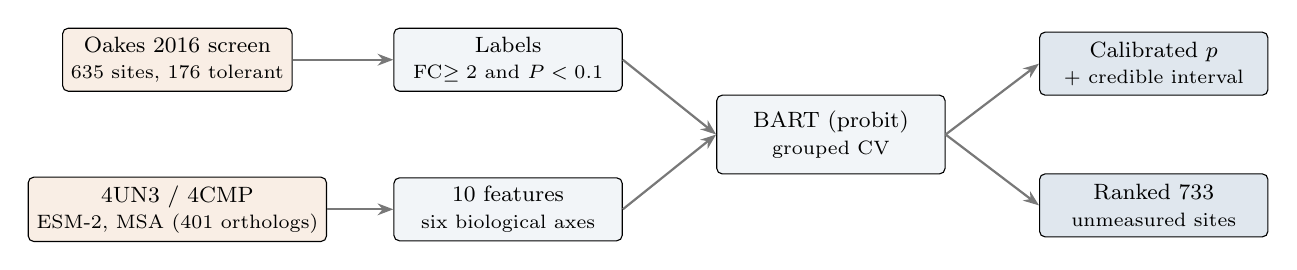
\begin{tikzpicture}[
  box/.style={draw, rounded corners=2pt, align=center, font=\footnotesize,
              minimum height=0.8cm, minimum width=2.9cm, inner sep=3pt, fill=accent!6},
  data/.style={box, fill=warm!10},
  outbox/.style={box, fill=accent!14},
  arr/.style={-{Stealth[length=2mm]}, soft, thick}]
  \node[data] (oakes) at (0,0.95)  {Oakes 2016 screen\\\scriptsize 635 sites, 176 tolerant};
  \node[data] (struct) at (0,-0.95) {4UN3 / 4CMP\\\scriptsize ESM-2, MSA (401 orthologs)};
  \node[box] (label) at (4.2,0.95) {Labels\\\scriptsize FC$\ge2$ and $P<0.1$};
  \node[box] (feat) at (4.2,-0.95) {10 features\\\scriptsize six biological axes};
  \node[box, minimum height=1.0cm] (model) at (8.3,0) {BART (probit)\\\scriptsize grouped CV};
  \node[outbox] (cal) at (12.4,0.9) {Calibrated $p$\\\scriptsize $+$ credible interval};
  \node[outbox] (rank) at (12.4,-0.9) {Ranked 733\\\scriptsize unmeasured sites};
  \draw[arr] (oakes) -- (label);
  \draw[arr] (struct) -- (feat);
  \draw[arr] (label.east) -- (model.west);
  \draw[arr] (feat.east) -- (model.west);
  \draw[arr] (model.east) -- (cal.west);
  \draw[arr] (model.east) -- (rank.west);
\end{tikzpicture}
\caption{Overview of the pipeline. A public functional screen provides the labels; structural and
sequence sources provide the features; a single BART classifier is evaluated under grouped
cross-validation and then applied to rank the 733 residues the screen did not measure.}
\label{fig:pipeline}
\end{figure}

\section{Data and its caveats}

The labels are derived from the Oakes et al.\ (2016) screen. The authors inserted an 86-residue
PDZ domain across Cas9, subjected the library to a CRISPRi functional selection using
catalytically dead Cas9, and sequenced the pool before and after selection. Functional variants
survive and become enriched, whereas non-functional variants are depleted. Each surviving position
is reported with a fold change, the ratio of its post-selection to its pre-selection abundance,
and an associated $P$-value.

Parsing the data required several deliberate decisions. The supplement contains only significant
entries (636 rows, maximum $P$ of 0.0996), so the $P<0.1$ threshold is the authors', not mine. I
removed the single row at \texttt{AA=0}, an insertion N-terminal to residue 1 with no residue to
map, which leaves 635 measured sites. Two clones are absent from the pre-screen library and report
infinite fold change; I treat them as strongly enriched. Site \texttt{AA=i} is mapped to the
features of residue $i$, the transposon's short duplication having already been collapsed into
SpCas9 numbering by the authors. The principal concern is coverage: the screen reached only about
70\% of positions, and the significant table is a subset of those, so 733 residues are unlabelled.
An unmeasured residue is not an intolerant one, and labelling these 733 as negatives would
fabricate data and degrade calibration. They are therefore withheld entirely and constitute the
prediction set that the model scores and the laboratory consumes.

\section{Target: binary, with a defended threshold}

I label a site tolerant when its fold change is at least 2 and its $P$-value is below 0.1. The
target is binary by design: the decision it supports is itself binary, namely whether or not to
attempt an insertion, and a calibrated probability is what allows a laboratory to rank and
threshold candidates. The two-fold cut is the conventional definition of meaningful enrichment; it
yields 176 positives out of 635, a base rate near 28\%. With ten features this corresponds to
roughly ten events per variable, a ratio that limits overfitting. A regression target on
\texttt{log2} fold change remains available as an alternative. It retains more information, but its
tails are poorly behaved (fold changes of zero and of infinity), and the operational question is
binary, so the binary target is primary.

\section{Features and why each should carry signal}

I selected ten features to characterise the environment of each residue, organised into six
biological axes; the grouping supports the rationale and importance reporting, while the model
receives only a flat ten-dimensional vector. Three features address whether there is physical room
for an insertion: relative solvent-accessible surface area, local atomic packing within 18\,\AA,
and the crystallographic B-factor. Two address disruption of nucleic-acid binding, the minimum
distances to the guide RNA and to the DNA, since the binding channels are selected against. One
addresses local rigidity, the distance to the nearest helix or strand terminus, which separates
tolerant element edges from rigid mid-element positions. Three address evolutionary constraint:
ESM-2 entropy, alignment conservation, and indel frequency, since positions that tolerate natural
indels tend to tolerate engineered insertions. The final axis addresses conformational dynamics.

The conformational-dynamics feature was added last and is the most mechanistically motivated.
SpCas9 undergoes a large conformational change upon activation, so an insertion in a region that
must move during that transition tends to abolish function. I quantify this by superposing the apo
(4CMP) and holo (4UN3) structures on the rigid RuvC core (261 residues, 2.37\,\AA\ RMSD) and
measuring the per-residue C$\alpha$ displacement between the two states. The separation between
classes is pronounced: tolerant sites move 14.6\,\AA\ on average, intolerant sites 26.9\,\AA.
Conservation is computed by two independent methods, the ESM-2 protein language model and a MAFFT
alignment of 401 orthologs, so that the resulting signal does not depend on either alone.

\section{Model}

I train a single model: a Bayesian Additive Regression Trees (BART) classifier with a probit link,
fitted with \texttt{dbarts}. The choice suits the data. With only 176 positives, a
self-regularising model is preferable to one requiring extensive tuning, and BART regularises
through priors on tree depth and leaf magnitude. As a sum of shallow trees, it also captures
nonlinearities and interactions without manual specification, which is relevant because several
features are non-monotonic; tolerated positions tend to lie a short distance from the DNA rather
than maximally far from it. Most importantly for this application, BART is Bayesian, so 1{,}000
posterior draws yield both a calibrated probability and a 95\% credible interval per residue.

\begin{figure}[h]
\centering
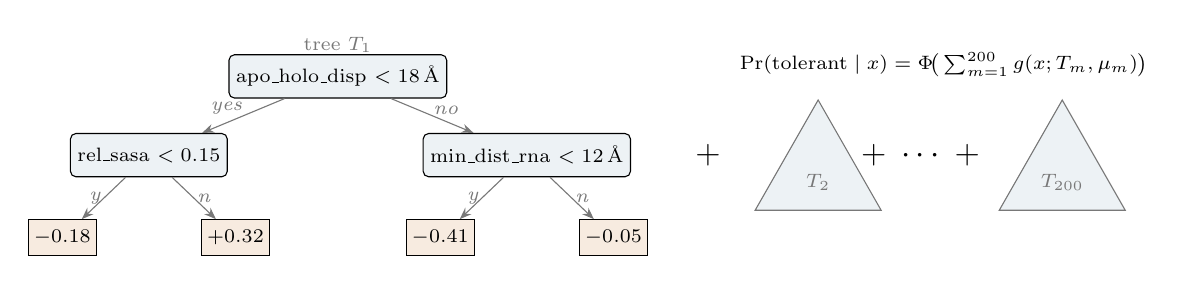
\begin{tikzpicture}[
  font=\footnotesize,
  dec/.style={draw, rounded corners=2pt, fill=accent!8, align=center,
              inner sep=2.5pt, font=\scriptsize, minimum height=0.55cm},
  leaf/.style={draw, fill=warm!12, align=center, inner sep=2pt, font=\scriptsize,
               minimum width=0.85cm, minimum height=0.46cm},
  edge/.style={-{Stealth[length=1.5mm]}, soft},
  elab/.style={font=\scriptsize\itshape, soft, inner sep=1pt}]
  \node[dec] (r)  at (0,2.1) {apo\_holo\_disp $< 18$\,\AA};
  \node[dec] (l1) at (-2.4,1.1) {rel\_sasa $< 0.15$};
  \node[dec] (r1) at (2.4,1.1) {min\_dist\_rna $< 12$\,\AA};
  \node[leaf] (ll) at (-3.5,0.05) {$-0.18$};
  \node[leaf] (lr) at (-1.3,0.05) {$+0.32$};
  \node[leaf] (rl) at (1.3,0.05)  {$-0.41$};
  \node[leaf] (rr) at (3.5,0.05)  {$-0.05$};
  \draw[edge] (r) -- (l1) node[elab, midway, above left=-1pt] {yes};
  \draw[edge] (r) -- (r1) node[elab, midway, above right=-1pt] {no};
  \draw[edge] (l1) -- (ll) node[elab, midway, left] {y};
  \draw[edge] (l1) -- (lr) node[elab, midway, right] {n};
  \draw[edge] (r1) -- (rl) node[elab, midway, left] {y};
  \draw[edge] (r1) -- (rr) node[elab, midway, right] {n};
  \node[soft, font=\scriptsize] at (0,2.5) {tree $T_1$};
  \node[font=\large] at (4.7,1.1) {$+$};
  \draw[soft, fill=accent!8] (5.3,0.4) -- (6.1,1.8) -- (6.9,0.4) -- cycle;
  \node[soft, font=\scriptsize] at (6.1,0.75) {$T_2$};
  \node[font=\large] at (7.4,1.1) {$+\;\cdots\;+$};
  \draw[soft, fill=accent!8] (8.4,0.4) -- (9.2,1.8) -- (10.0,0.4) -- cycle;
  \node[soft, font=\scriptsize] at (9.2,0.75) {$T_{200}$};
  \node[align=center, font=\scriptsize] at (7.7,2.25)
    {$\Pr(\text{tolerant}\mid x)=\Phi\!\big(\sum_{m=1}^{200} g(x;T_m,\mu_m)\big)$};
\end{tikzpicture}
\caption{Structure of the BART model. The latent score for a residue is the sum of 200 shallow
trees, mapped through the probit link $\Phi$ to a probability. The example tree $T_1$ splits first
on conformational displacement, then on exposure or proximity to the guide RNA; positive leaf
values increase the predicted tolerance. Posterior draws over the ensemble yield the per-residue
credible interval.}
\label{fig:tree}
\end{figure}

The depth prior restricts trees to two or three levels and the leaf prior ($k=2$) shrinks their
contributions, so at this sample size the regularisation dominates and the ensemble does not
overfit. I verified this rather than assuming it. A small grid over the leaf-shrinkage and
tree-count parameters changed the honest out-of-fold score by at most 0.02, and the optimism gap,
the difference between the best inner-loop score and the honest out-of-fold score, was only 0.073.
A gap this small indicates that further search would fit cross-validation noise rather than signal,
so the defaults were retained ($k=2$, \texttt{ntree}$=200$, 1{,}000 draws).

\section{Honest evaluation}

Residues are spatially autocorrelated, since positions adjacent along the chain resemble one
another, so a random $k$-fold split leaks neighbouring residues across the train-test boundary and
inflates apparent performance. I therefore use two grouped splits that bracket the deployment
regime. Block cross-validation partitions the sequence into eight contiguous segments,
approximating the setting in which scored residues are interspersed among measured ones.
Leave-a-domain-out cross-validation withholds an entire Cas9 domain at a time, a stricter test of
generalisation to unseen structure. AUPRC is the primary metric, because the classes are imbalanced
and it reflects the quality of the ranked shortlist the laboratory acts upon; precision in the top
20 and top 50 is reported for the same reason. Accuracy is uninformative here, as predicting
``intolerant'' for every residue already attains 72\%.

\begin{table}[h]
\centering
\caption{Out-of-fold performance of the final BART model (ten features), base rate 0.28. The two
schemes bracket deployment, and their close agreement says the model is not leaning on shortcuts
tied to which domain a residue sits in.}
\label{tab:perf}
\begin{tabular}{lcccccc}
\toprule
Cross-validation scheme & $n_{\text{OOF}}$ & AUPRC & AUROC & P@20 & P@50 & Brier \\
\midrule
Leave-a-domain-out (strict) & 627 & \textbf{0.637} & 0.809 & 0.70 & \textbf{0.82} & 0.149 \\
Contiguous block            & 635 & 0.645 & 0.837 & --   & --   & --    \\
\bottomrule
\end{tabular}

{\footnotesize\itshape P@$k$ and Brier are for the headline (domain) run; block is shown for the
robustness comparison.}
\end{table}

The progression toward these results is informative. The headline AUPRC increased from 0.50 to
0.59 to 0.64 across three rounds of feature work, none of it attributable to tuning
(Figure~\ref{fig:progress}). The first gain followed the removal of a leaking feature; the second
followed the removal of two redundant features and the addition of the dynamics feature. Against a
base rate of 0.28, the final model places 41 of its 50 highest-ranked sites on genuinely tolerant
residues.

\begin{figure}[h]
\centering
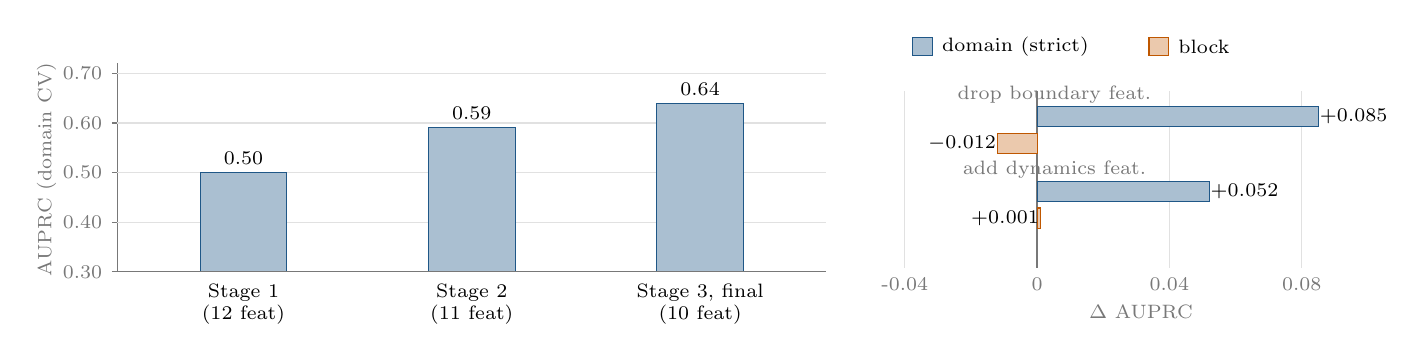
\begin{tikzpicture}[font=\footnotesize]
  \def\sca{6.3}
  \draw[soft] (0,0) -- (0,2.65);
  \foreach \v in {0.30,0.40,0.50,0.60,0.70}{
    \pgfmathsetmacro\yy{(\v-0.30)*\sca}
    \draw[soft] (-0.07,\yy) -- (0,\yy) node[left, xshift=-2pt, font=\scriptsize]{\v};
    \draw[soft!22] (0,\yy) -- (9.0,\yy);
  }
  \node[rotate=90, soft, font=\scriptsize] at (-0.9,1.3) {AUPRC (domain CV)};
  \foreach \cx/\bt/\lab in {1.6/0.50/{Stage 1\\(12 feat)},
                            4.5/0.59/{Stage 2\\(11 feat)},
                            7.4/0.64/{Stage 3, final\\(10 feat)}}{
    \pgfmathsetmacro\ybt{(\bt-0.30)*\sca}
    \fill[accent!38, draw=accent] (\cx-0.55,0) rectangle (\cx+0.55,\ybt);
    \node[font=\scriptsize] at (\cx,\ybt+0.18) {\bt};
    \node[align=center, font=\scriptsize, below=1pt] at (\cx,0) {\lab};
  }
  \draw[soft] (0,0) -- (9.0,0);
  % leakage panel
  \begin{scope}[xshift=10.0cm, yshift=0.15cm]
    \def\scb{42.0}
    \pgfmathsetmacro\zero{(0+0.04)*\scb}
    \foreach \d in {-0.04,0,0.04,0.08}{
      \pgfmathsetmacro\xx{(\d+0.04)*\scb}
      \draw[soft!22] (\xx,-0.1) -- (\xx,2.15);
      \node[soft, font=\scriptsize, below] at (\xx,-0.1) {\d};
    }
    \draw[soft, thick] (\zero,-0.1) -- (\zero,2.15);
    \node[soft, font=\scriptsize, below] at (3.0,-0.45) {$\Delta$ AUPRC};
    \foreach \cy/\dom/\blk/\dlab/\blab in {%
        1.65/0.085/-0.012/{$+0.085$}/{$-0.012$},
        0.7/0.052/0.001/{$+0.052$}/{$+0.001$}}{
      \pgfmathsetmacro\xd{(\dom+0.04)*\scb}
      \pgfmathsetmacro\xk{(\blk+0.04)*\scb}
      \fill[accent!38,draw=accent] (\zero,\cy+0.04) rectangle (\xd,\cy+0.3);
      \fill[warm!32,draw=warm]    (\zero,\cy-0.3) rectangle (\xk,\cy-0.04);
      \node[font=\scriptsize] at (\xd+0.45,\cy+0.17) {\dlab};
      \node[font=\scriptsize] at (\xk-0.45,\cy-0.17) {\blab};
    }
    \node[soft, font=\scriptsize, align=center] at (1.9,2.1) {drop boundary feat.};
    \node[soft, font=\scriptsize, align=center] at (1.9,1.15) {add dynamics feat.};
    \fill[accent!38,draw=accent] (0.1,2.6) rectangle (0.35,2.82);
    \node[right, font=\scriptsize] at (0.35,2.71) {domain (strict)};
    \fill[warm!32,draw=warm] (3.1,2.6) rectangle (3.35,2.82);
    \node[right, font=\scriptsize] at (3.35,2.71) {block};
  \end{scope}
\end{tikzpicture}
\caption{Left: headline AUPRC increases with feature work, not with tuning. Right: the leakage
test. Dropping \texttt{dist\_to\_domain\_boundary} improves the strict split ($+0.085$) but not the
block split ($-0.012$), the signature of a feature that implicitly encodes domain identity. The
dynamics feature shows the opposite pattern, improving the strict split.}
\label{fig:progress}
\end{figure}

\section{What the model learned, and a detected leakage}

Aggregated by axis, BART's variable inclusion ranks exposure first ($\approx0.30$), followed by
proximity to the nucleic acids ($\approx0.20$), conservation ($\approx0.20$), and dynamics
($\approx0.10$). This ordering is consistent with the biology: a favourable insertion site has
available room, lies away from the binding channels, is not part of a conserved core, and is not
required to move during activation. The leakage test corrected an initial assumption. The feature
\texttt{dist\_to\_domain\_boundary}, added on biological grounds, implicitly encodes the domain to
which a residue belongs. Removing it changed the block score negligibly ($-0.012$) but raised the
strict leave-a-domain-out score by 0.085 (Figure~\ref{fig:progress}, right). This asymmetry, a
benefit when the domain is represented in training and a penalty when it is not, is the
characteristic signature of leakage, and the feature was removed. The dynamics feature exhibits the
opposite pattern and was retained. Ablation determined the remaining selections
(Table~\ref{tab:ablation}): univariate strength does not imply marginal value, so features were
retained by their marginal contribution rather than by their performance in isolation.

\begin{table}[h]
\centering
\caption{Feature ablation under leave-a-domain-out CV (gradient-boosting proxy). Production
features baseline AUPRC 0.558. Positive drop-one and add-one values mean the feature helps. The
retained dynamics feature is marked; several mechanism-driven candidates were rejected.}
\label{tab:ablation}
\scriptsize
\begin{tabular}{llcc@{\hskip 1.1em}llcc}
\toprule
Feature & Group & Univar. & Drop1 & Feature & Group & Univar. & Add1 \\
\midrule
min\_dist\_rna     & prod & 0.545 & $+0.003$ & solvent\_cone        & novel & 0.502 & $+0.001$ \\
flexibility        & prod & 0.516 & $+0.002$ & min\_dist\_heterodup. & novel & 0.482 & $-0.006$ \\
open\_volume\_18A  & prod & 0.455 & $-0.006$ & contact\_order       & novel & 0.452 & $+0.001$ \\
rel\_sasa          & prod & 0.448 & $-0.008$ & \textbf{apo\_holo\_disp} & \textbf{novel} & 0.394 & $\mathbf{+0.018}$ \\
indel\_frequency   & prod & 0.363 & $+0.002$ & long\_range\_contacts & novel & 0.379 & $-0.013$ \\
dist\_to\_sse\_end & prod & 0.347 & $-0.008$ & min\_dist\_na\_ends   & novel & 0.357 & $+0.009$ \\
msa\_conservation  & prod & 0.319 & $\mathbf{+0.038}$ & min\_dist\_nontarget & novel & 0.344 & $-0.019$ \\
esm2\_entropy      & prod & 0.295 & $-0.010$ & true\_insertion\_freq & novel & 0.237 & $-0.020$ \\
\bottomrule
\end{tabular}
\end{table}

A normal-mode elastic-network model was tested as an alternative dynamics descriptor: using ProDy,
I built an Anisotropic Network Model on the holo C$\alpha$ trace and took each residue's
fluctuation in the ten slowest collective modes (\texttt{anm\_msf}). Although it covers every
resolved residue, it did not help, lowering AUPRC slightly under both schemes (0.635 to 0.621 under
leave-a-domain-out, 0.645 to 0.639 under block) and performing clearly worse as a substitute for
\texttt{apo\_holo\_disp} (0.575 under leave-a-domain-out). The model reports the intrinsic
equilibrium fluctuations of a single wild-type structure, a smooth profile dominated by termini and
surface loops, so it overlaps the existing B-factor feature and is far less specific to the
apo-to-holo activation motion that \texttt{apo\_holo\_disp} captures directly from two distinct
states.

Two further failure modes should be noted. The non-monotonic dependence on distance to DNA is only
partially captured, and a decomposition into specific channel distances did not improve on the
broad feature.

\section{Limitations}

The metrics are optimistic by construction, since training and evaluation are restricted to
significant sites; the 0.82 top-50 precision is a ceiling on a clean subset rather than a
deployment guarantee, and only experimental validation can establish the true operating point.
Confidence intervals on the deltas were not computed, and with six folds and 176 positives a
difference such as 0.64 versus 0.59 is partly noise. The dynamics feature is roughly one-third
imputed (residues unresolved in the apo structure), with non-random missingness, so part of its
value may be artefactual. RuvC is discontinuous in sequence, so only HNH, PI, and REC are genuinely
unseen-domain holdouts. Finally, this concerns a single inserted domain in a single host protein
scored against static crystal structures, so generalisation to other inserts is untested.

\section{What I would do next}

With additional time, the highest-value addition is a feature that directly simulates the
insertion: folding local Cas9-PDZ chimera windows with ESMFold and reading the predicted confidence
(pLDDT) over the Cas9 flank, the one descriptor that models the grafted domain rather than its
environment. I would also add bootstrap confidence intervals to the feature deltas. With more data,
the next step is prospective validation: testing the highest-ranked sites at the bench,
recalibrating on the results, and adding a \texttt{log2}-fold-change regression head for finer
ranking.

\end{document}
